% Chapter 3

\chapter{The \alphat Search} % 

\label{Chapter3} % For referencing the chapter elsewhere, use \ref{Chapter1} 

\lhead{Chapter 3. \emph{The \alphat Search}} % This is for the header on each page - perhaps a shortened title

%----------------------------------------------------------------------------------------

\section{\boldsymbol{\alphat}}
Large SM backgrounds are caused by vector boson decays to neutrinos and mismeasured QCD. Calculating missing energy requires precise information from each of the calorimeters, tracking and muon subdetectors. This can easily lead to fake missing energy in the final state from mismeasured QCD jets \cite{randall}. Such a source can be particularly expected in the uncertain environment just after turn on.  The $\alpha_T$ variable has been designed explicitly to remove this source of background and is defined in equation \ref{alph}.
\begin{equation}
\label{alph}
\alpha_T=\frac{1}{2}\frac{1-(\Delta H_T/H_T)}{\sqrt{1-(\cancel{H_T}/H_T)^2}}
\end{equation}
This is defined for n-jets by creating a pseudo di-jet system which minimises the difference in energy between the two pseudo jets ($\Delta H_T$) in the event. The total transverse energy is defined as $H_T=\sum_{i=1}^n|p_t^{j_i}|$ and the mising energy $\cancel{H_T}=|{\sum_{i=1}^n p_T^{j_i}}|$. In the case of jet mismeasurement or neutrinos from heavy flavour jets the energy imbalance $\Delta H_T$ and missing energy $\cancel{H_T}$ are highly correlated and $\alpha_T<0.5$. A dedicated study is required to find the threshold beyond which QCD backgrounds are negligible. In the previous $\alpha_T$ search the cut was at $\alpha_T<0.55$. A sample distribution of $\alpha_T$ from this search is shown in figure \ref{alphdis} \cite{CMSAT8}.
\begin{figure}
\centering
    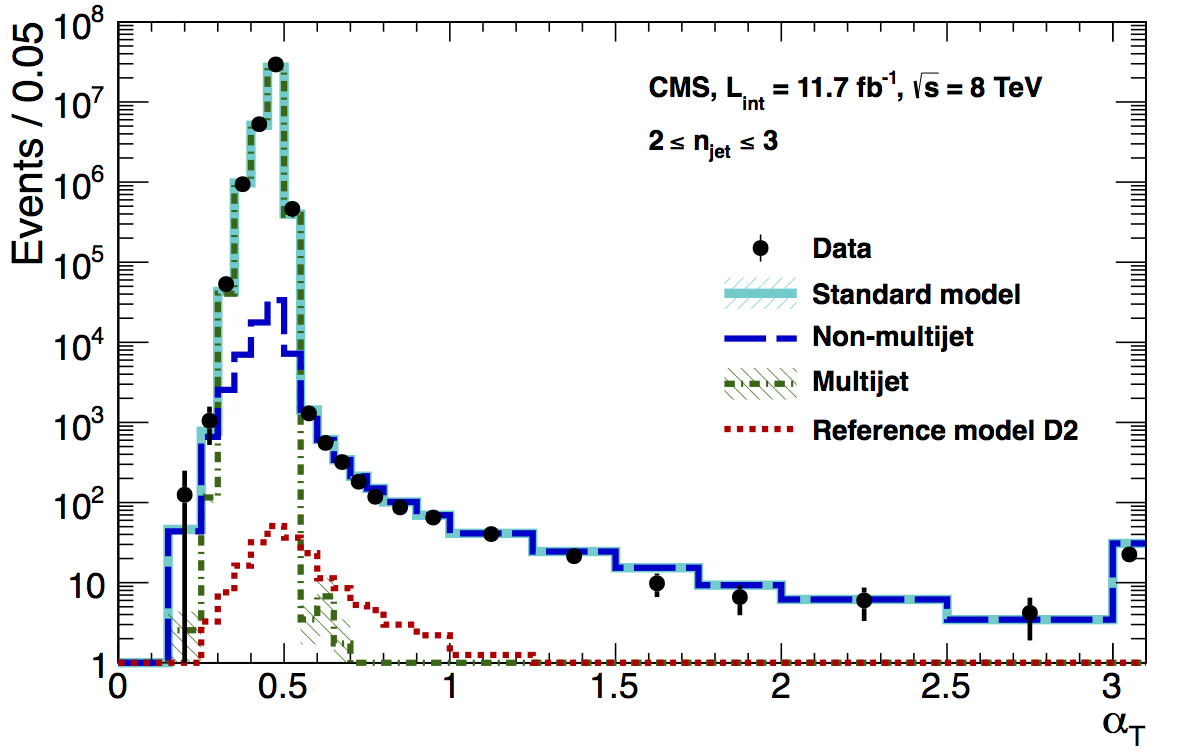
\includegraphics[width=0.8\textwidth]{Figures/sample_aT.jpg}
  \caption{$\alpha_T$ distribution shown for a particular search region. The contribution from a SUSY reference model shows events above 0.55.}
  \label{alphdis}
\end{figure}

\subsection{Event Selection}
In order to reduce backgrounds from electroweak processes with isolated leptons are vetoed. A pure multijet topology is ensured by additionally vetoing events with isolated photons. Events are categorised according the jet multiplicity and btag (number of jets originating from b quarks). Selected events are required to have $\scalht > 200 GeV$ and at least two jets with $p_T > 100GeV$ and the remainder $p_T > 40GeV$. A new asymmetric category has been added to increase sensitivity to monojet like topologies. In this case the lead jet has $p_T > 100 GeV$ and all remaining jets satisfy $100 GeV > p_T > 40GeV$. All jets must have $\eta < 2.4$.

In order to maximise acceptance the \alphat thresholds are chosen in each \scalht bin as the minimum required for effective QCD rejection as well as to be efficient after trigger requirements. The thresholds chosen are shown in \ref{}. These are designed to reduce QCD contamination to the sub percent level (a dedicated study is required with data). The sensitivity of each bin is then optimised (see \ref{}). 


\subsection{Background Estimation}
The remaining background from electroweak processes must be estimated. The dominant backgrounds are vector boson and top pair production in association with jets. To minimise dependence on Monte Carlo a data driven approach is taken. The number of events in control regions with low signal contamination is measured. Then the effect in the signal region is predicted using equation \ref{control}. To understand the systematic error on these predictions closure tests are carried out whereby one control sample is used to predict another. Using an ensemble of such tests (binned in \scalht and categories) allows an estimation of the size of any systematic in each bin.

\begin{equation}
\label{control}
N_{pred}^{signal}=\frac{N_{MC}^{signal}}{N_{MC}^{control}}\times N^{control}_{obs}
\end{equation} 

% \subsection{Interpretation}
% Finally the data from CMS must be interpreted. This is done using simplified models which have only one production and decay mode and are a measure of the reach of a search in parameter space. Two sample simplified model decays from the latest 8 TeV $\alpha_T$ analysis involving decays to quarks are shown in figure \ref{simp}. Each simplified model is suited to a different signal bin. The model predictions for different parent and LSP masses are then confronted with the background estimation along with the data to make mass exclusion planes. These are shown in figure \ref{simp2} for the latest search.
% \begin{figure}
% \hfill
% \subfigure[Squark Production (T1)]{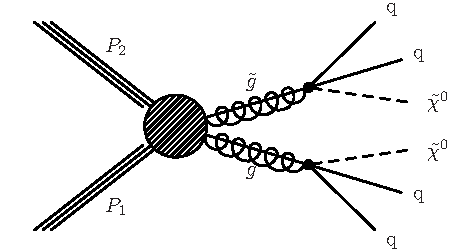
\includegraphics[width=5cm]{Figures/T1}}
% \hfill
% \subfigure[Gluino Production (T2)]{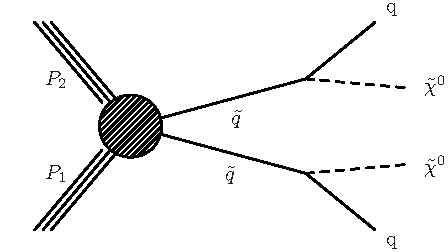
\includegraphics[width=5cm]{Figures/T2}}
% \hfill
% \caption{Two typical simplified models involving gluino and squark decays to quarks}
% \label{simp}
% \end{figure}
% \begin{figure}
% \hfill
% \subfigure[T1 Exclusion]{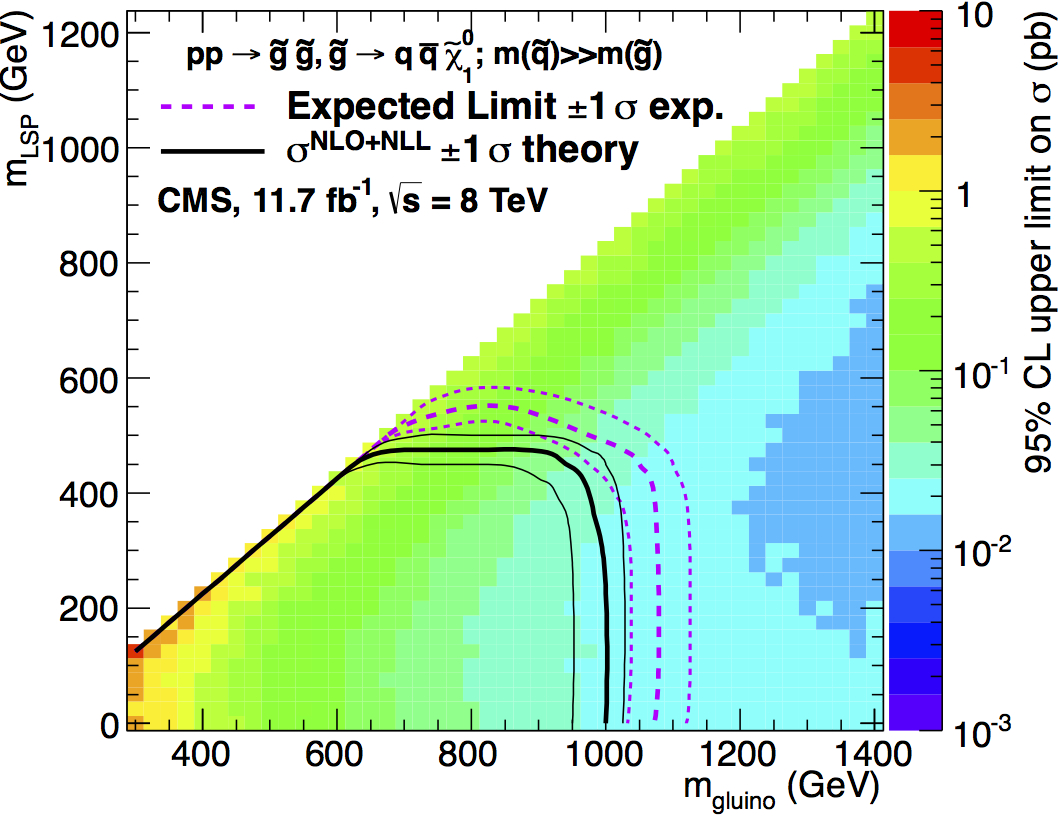
\includegraphics[width=7cm]{Figures/T1plot}}
% \hfill
% \subfigure[T2 Exclusion]{\includegraphics[width=7cm]{Figures/T2plot}}
% \hfill
% \caption{Exclusion planes for two simplified models}
% \label{simp2}
% \end{figure}
